%% Example of a LaTeX source file for a COLING-2012 submission
%% last updated: July 10, 2012
%% Optional instructions for authors within the tex file are provided as comments and start with 'for authors:...'
\documentclass[10pt,a5paper,twoside]{article}
\usepackage{coling2012}
\usepackage{comment}
%\title{Translating to Shakespeare: A Case Study in Paraphrasing Writing Styles}
\title{You can be Shakespeare! \\ A Case Study in Paraphrase Targeting Writing Styles}
%for authors: in case of more than four author names ref. to commented line below 
%\author{$Annie~SMITH^{1, 2}~~~LI~Xiao Dong^{1, 3}$\\$~~~Third~Author^{1, 2}~~~Fourth~Author^{1, 3}~~~ Fifth~Author^{2, 3}$\\
\author{$Author1^{1, 2}~~~Author2^{1, 3}$\\
{\small  	(1) INSTITUTE\_1, address 1\\ 
 		(2) INSTITUTE\_2, address 2\\
		(3) INSTITUTE\_3, address 3\\
  \texttt{author1@institute1, author@institute2} \\ 
}}

\begin{document}
\maketitle
%% The first mandatory ABSTRACT (\abstractEn) section below is for the English language
\abstractEn{  %ABSTRACT}{
We present initial investigation into the task of paraphrasing language while targeting a particular writing style.
The plays of William Shakespeare and their modern translations are used as a testbed for evaluating
paraphrase systems targeting a specific style of writing.
%We demonstrate that existing evaluation metrics developed in the Machine Translation and Paraphrase communities are
%insufficient when the goal is to generate paraphrases targeting a specific style, and
%propose a series of new metrics to measure how closely the generated paraphrases match the target
%style.  
We show that even with a relatively small amount of parallel training data available, it is
possible to learn paraphrase models which capture stylistic phenomenon, and these models outperform
baselines based on dictionaries and out-of-domain parallel text.
In addition we present an initial investigation into automatic evaluation metrics for paraphrasing writing style.
To the best of our knowledge this is the first work to investigate the task of
paraphrasing text with the goal of targeting a specific style of writing.
}

\keywordsEn{Paraphrase, Writing Style}

\section{Introduction}
%The plays of William Shakespeare and their \emph{modern} translations are treated
%as parallel text which is used to learn paraphrase models targeting the style of Early Modern English employed by Shakespeare.

Identical meaning can be expressed or \emph{paraphrased} in many different ways; automatically detecting or generating different expressions with the same meaning is 
fundamental to many natural language understanding tasks \cite{Giampiccolo07}, so much previous work has investigated methods for automatic paraphrasing \cite{Barzilay03,dolan04,Shinyama03,Das09,bannard05}.  
Although two utterances may be semantically equivalent, they can still be stylistically quite different.  For example, the same information
is likely to be conveyed using very different lexical and grammatical patterns in advertising materials v.s. technical manuals, or in Shakespearean plays v.s. Hollywood movies.

In this paper, we investigate the task of automatic paraphrasing when targeting a writing style, focusing specifically on the style of Early Modern English employed by William Shakespeare.
We exploit modern translations of 17 plays written to help students better understand Shakespeare's work.  A parallel corpus is extracted from these modern translations,
which is then used to train phrase-based translation models which are capable of automatically paraphrasing ordinary sentences into Shakesperean English.  In addition we develop several
baseline systems which don't make use of this source of parallel text and instead rely on dictionaries of expressions commonly found in Shakesperean english, or parallel monolingual text
gathered through crowd sourcing platforms such as Amazon's Mechanical Turk \cite{chen11}.

We evaluate these models both through human judgements and standard evaluation metrics from the Machine Translation and paraphrase literature, however no previous work has investigated the ability of these automatic metrics
to capture the notion of writing style.  We propose several new metrics for evaluating paraphrases targeting a specific writing style, and measure correlation with human judgements showing  promising, yet
preliminary results.

Systems which are capable of automatically paraphrasing literary writing styles could be directly beneficial for educational applications, for example helping students to experiment with writing literature in the
style of authors they are studying.  Additionally note that out of the 37 surviving plays written by William Shakespeare, only 17 currently have modern translations available; although we have not yet formally evaluated
paraphrasing in the other direction, we believe this work also has the potential to make the other 20 plays more accessible to students of Shakespeare by automatically generating relatively high-quality modern translations.

\begin{comment}
\begin{itemize}
  \item Define what we mean by writing styles.
  \item Define the paraphrasing task and describe previous work.
  \item Motivate the need for paraphrasing targeting a specific writing style (e.g. students of literature in a specific style, or helping people to understand documents written in an esoteric style).
   \begin{itemize}
     \item Mention several domains where paraphrasing into/out of a specific writing style could be beneficial (e.g. technical manuals, legal documents, etc...)
   \end{itemize}
  \item Summarize the main contributions.
\end{itemize}
\end{comment}

\section{Data}
We propose to use Shakespeare's plays as a testbed for the task of paraphrasing while targeting a specific writing style.  Because these plays are some of the
highest regarded examples of English literature and are also very unique in style, many linguistic resources are available such as parallel corpora
of modern translations and dictionaries of stylistically representative words and their modern equivalents.

We compare 3 different stylistic paraphrase systems targeting Shakesperean English.  One which leverages parallel corpora of modern translations, another which makes use
of dictionaries of stylistically representative expressions, and another which leverages out-of-domain monolingual parallel data.

\subsection{Modern Translations}
Having access to parallel text in the target style allows us to train statistical models for generating paraphrases, and also perform automatic evaluation of semantic adequacy using BLEU, which requires access to a set of reference translations.  For this purpose we scraped modern translations of 17 Shakespeare plays from \url{http://nfs.sparknotes.com}, and an additional 8 translations of overlapping plays from \url{http://enotes.com}, giving us two reference translations for 8 out of the 17 plays.

After tokenizing and lowercasing, the plays were aligned using Bob Moore's bilingual sentence \cite{Moore02} aligner, which produced about 21,079 alignments out of 31,718 sentences in the Sparknotes data, and 10,365 sentence pairs out of 13,640 sentences in the Enotes data.  The modern translations from each source are qualitatively quite
different.  The Sparknotes paraphrases tend to differ significantly from the original text, whereas the Enotes translations are much more conservative, making fewer changes.
To illustrate these differences empirically and provide an initial paraphrase baseline, we computed BLEU scores of the unchanged modern translations against Shakespeare's 
original text; the Sparknotes paraphrases result in a BLEU score of 24.67, whereas the Enotes paraphrases prouce a much higher BLEU of 52.30 indicating their similarity to the original text.
These corpus statistics are summarized in table \ref{corpus_stats}.

\begin{table}
  \begin{center}
    \begin{tabular}{|l|r|r|r|}
      \hline
      corpus & initial size & aligned size & No-Change BLEU\\
      \hline
      \hline
      \url{http://nfs.sparknotes.com} & 31,718 & 21,079 & 24.67 \\
      \hline
      \url{http://enotes.com} & 13,640 & 10,365 & 52.30 \\
      \hline
    \end{tabular}
  \end{center}
  \caption{Parallel corpora generated form modern translations of Shakespeare's plays}
  \label{corpus_stats}
\end{table}

\subsection{Baselines} po
Phrase-based translation has been demonstrated to be an effective approach to generating paraphrases \cite{chen11,quirk04}, however this approach does require the existence of
parallel corpora which may not be available for many writing styles.  For this reason we were motivated to investigate alternative approaches.

\subsubsection{Dictionary Based Paraphrase}
\label{dictionary_baseline}
Several dictionaries of stylistically representative words of Shakesperean English and their modern equivalents are available on the web.  These dictionaries can be used 
to define a translation model which is used in combination with a language model as in standard phrase-based MT \cite{Koehn00}.

We gathered a set of 20,138 dictionary entries which were scraped from \url{http://www.shakespeareswords.com/}, then used heuristic rules to extract 68,709 phrase/word pairs.  Example
dictionary entries are presented in table \ref{dictionary_example}. As described in \cite{Koehn00}, we estimate phrase translation probabilities based on the frequencies of the translation words/phrases in the target language - the Shakespearean English. 

For instance, if we look at the modern English (*probably define EME, Shakespearean, modern/ordinary etc ... I don't know what words to use) word \emph{maybe}, our dictionary lists 4 possible Shakespearean translations. We can obtain the following conditional probabilities for each translation according to the n-gram back off model built on Shakespeare's 36 plays by SRILM toolkit (*ref "SRILM an Extensible Language Modeling Toolkit":



{\bf TODO:} need to describe how parameters were learned and combined with LM

\begin{table}
  \begin{center}
  \begin{tabular}{|l|l|}
    \hline
    target & source \\
    \hline
    \hline
    CRAVE & beg, entreat, request \\
    \hline
    GAGE & pledge, challenge \\
    \hline
    HAPLY & perhaps, maybe, by chance, with luck \\
    \hline
  \end{tabular}
  \end{center}
  \caption{Example dictionary entries}
  \label{dictionary_example}
\end{table}

\begin{table}
  \begin{center}
  \begin{tabular}{|l|l|||}
    \hline
    conditional probability & target & source \\
    \hline
    \hline
    0.0000790755 & PERCHANCE & maybe \\
    \hline
    0.00003691883 & PERADVENTURE & maybe \\
    \hline
    0.00007524298 & HAPLY & maybe \\
    \hline
    0.00007141065 & HAPPILY & maybe \\
    \hline
  \end{tabular}
  \end{center}
  \caption{Word frequency in target language}
  \label{word_frequency}
\end{table}



\subsubsection{Out of Domain Monolingual Parallel Data}
As a final baseline we consider a paraphrase system which is trained on out-of-domain parallel data gathered by asking users of Amazon's Mechanical Turk Service 
\cite{Snow08} to describe videos \cite{chen11}.  (*Maybe describe a bit more of the strength of Chen et al.'s data?) We combine a phrase table extracted from this out-of-domain parallel text, with an in-domain
language model consisting of Shakespeare's 37 (*should be 36? hold out) plays.  Although this monolingual parallel data does not include text in the target writing style,
the in-domain language model does bias the generated sentences towards Shakespeare's writing style.

\subsection{Comparison Using Existing Automatic Evaluation Metrics}
Figure \ref{bleupinc} compares a variety of sytstems targeting Shakesperean English using previously the previosly proposed BLEU \cite{Papineni02} and PINC \cite{chen11} automatic evaluation metrics.  A summary of each system is presented in table \ref{systems}.  Notice that the enotes data is quite similar to the original translations,
obtaining a BLEU score of 52.3 when compared against the original text.  Our goal is to produce paraphrases which make many changes to the input, therefore
in the remainder of this paper, we focus our evaluation on the Sparknotes data for evaluation.

Two main trends emerge from figure \ref{bleupinc}.  First, notice that all of the systems which are trained using parallel text achieve higher BLEU scores than the baseline
of not making any changes to the modern translations.  While the dictionary baseline achieves a competitive PINC score, indicating it is making significant changes to the 
input, it's BLEU is lower than the \emph{no changes} baseline.  Secondly, it seems apparent that the systems whose parameters are learned using Minimum Error Rate training
tend to be more conservative, making fewer changes to the input and thus achieving lower PINC scores, but not seeing any BLEU improvements on the test data.  Finally
we note that using the larger language model seems to yield a slight improvement in BLEU score.

\begin{table}
  \begin{center}
    \begin{tabular}{|l|p{3in}|}
      \hline
      System & Description \\
      \hline
      \hline
      16and7plays\_36LM & Phrase table learned from all 16 Sparknotes plays (other than R\&J) and language model built from all 36 of Shakespeare's plays, excluding R\&J.
      Uses default Moses parameters. \\
      \hline
      16and7plays\_36LM\_MERT & Same as 16and7plays\_36LM except parameters are tuned using Minimum Error Rate Training instead of using the default Moses parameters.\\
      \hline
      16and7plays\_16LM & Phrase table is built from both Sparknotes and Enotes data, and Language model is built from the 16 with modern translations\\
      \hline
      16and7plays\_16LM\_MERT & Same as 16and7plays\_16LM except parameters are tuned using MERT. \\
      \hline
      16plays\_36LM & Only Sparknotes modern translations are used.  All 36 plays are used to train Shakesperean language model. a\\
      \hline
      16plays\_36LM\_MERT & Same as 16plays\_36LM except parameters are tuned using MERT. \\
      \hline
      modern (no change) & No changes are made to the input, modern translations are left unchanged. \\
      \hline
      Dictionary & Dictionary baseline described in section \ref{dictionary_baseline}\\
      \hline
    \end{tabular}
  \end{center}
  \caption{Descriptions of various systems for Shakesperean Paraphrase.  Romeo and Juliet is held out for testing.}
  \label{systems}
\end{table}

\begin{figure}
  \begin{center}
    \begin{tabular}{cc}
      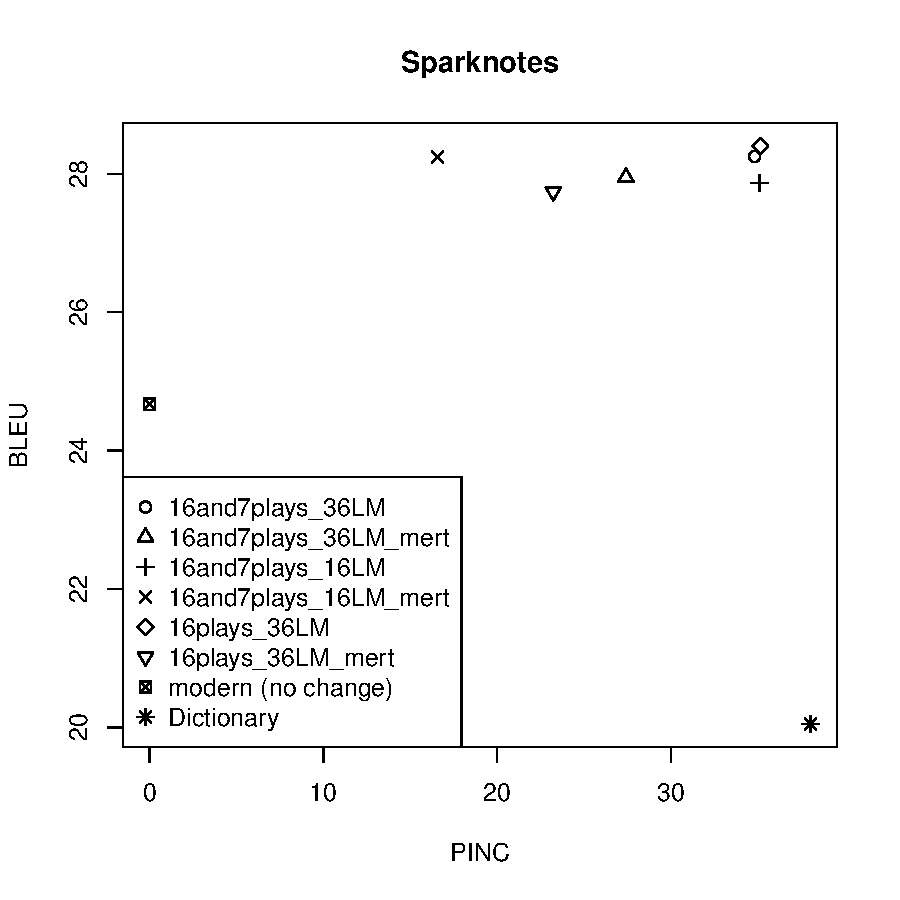
\includegraphics[width=2.4in]{figures/bleupinc1.pdf} & 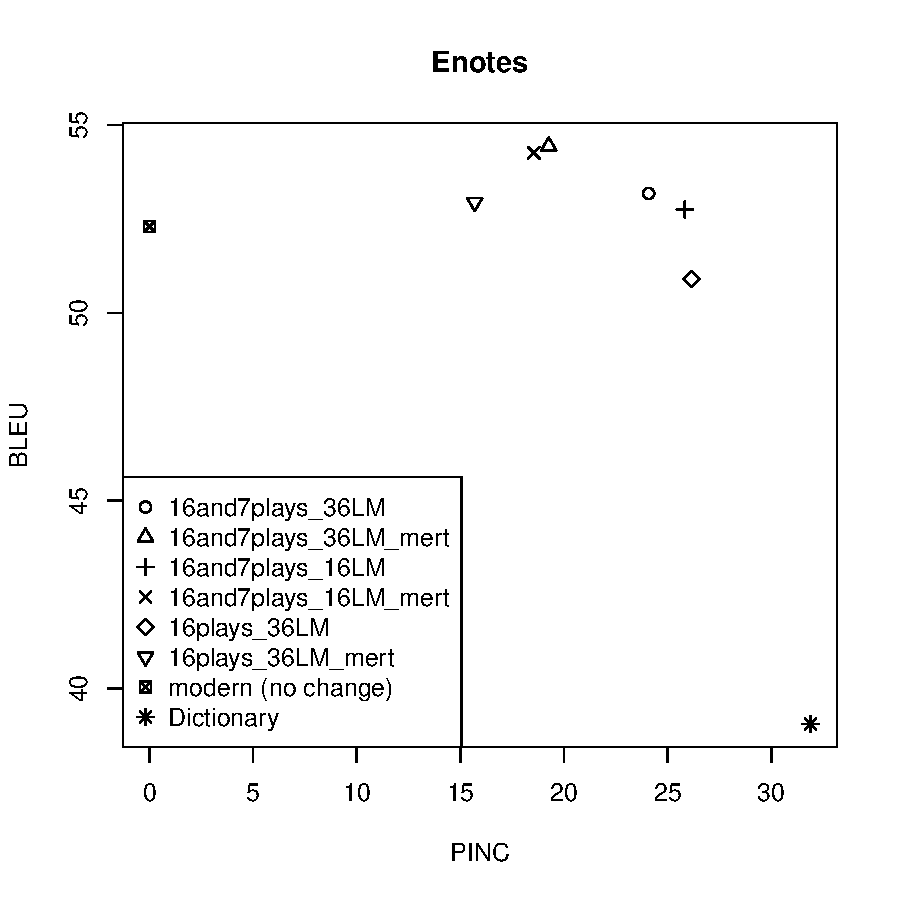
\includegraphics[width=2.4in]{figures/bleupinc2.pdf} \\
    \end{tabular}
  \end{center}
  \caption{Various Shakesperean Paraphrase systems compared using BLEU and PINC.}
  \label{bleupinc}
\end{figure}

Several example paraphrases generated by our system, both from Romeo and Juliet and several Hollywood movies are presented in table \ref{examples}.

\begin{table}
  \begin{center}
    \begin{tabular}{|l|l|p{1.4in}|p{1.4in}|}
      \hline
      Source & Speaker & Input & Output \\
      \hline
      \hline
      Romeo \& Juliet & Benvolio & he killed your relative , brave mercutio , and then young romeo killed him . & he slew thy kinsman , brave mercutio , and then young romeo kill him . \\
      \hline
      Romeo \& Juliet & Romeo & i can read my own fortune in my misery . & i can read mine own fortune in my woes . \\
      \hline
      Star Wars & Palpatine & If you will not be turned, you will be destroyed! & if you will not be turn 'd , you will be undone ! \\
      \hline
      Star Wars & Luke & Father, please! Help me! & father , i pray you , help me ! \\    
      \hline
      The Matrix & Agent Smith & Good bye, Mr. Anderson. & fare you well , good master anderson . \\
      \hline
      The Matrix & Morpheus & I'm trying to free your mind, Neo. But I can only show you the door. You're the one that has to walk through it. & i 'll to free your mind , neo. but i can but show you the door. you 're the one that hath to tread it . \\
      \hline
      Raiders of the Lost Ark & Belloq & Good afternoon, Dr. Jones. & well met , dr. jones . \\
      \hline
      Raiders of the Lost Ark & Jones & I ought to kill you right now. & i should kill thee straight . \\
      \hline
    \end{tabular}
  \end{center}
  \caption{Example Shakesperean paraphrases generated by the best overall system.}
\end{table}

\section{Evaluation Metrics}
\begin{itemize}
  \item Describe the need for automatic evaluation metrics.
  \item Describe previously used evaluation metrics for paraphrase.
  \item Highlight problems with previous metrics when targeting a specific writing style.
  \item Propose new metrics.
\end{itemize}

\section{Experiments}
\begin{itemize}
  \item Experimental setup.
  \item Present results from human evaluation comparing various systems.
  \item Analyze correlation between evaluation metrics and human judgments.
\end{itemize}

\section{Related Work}
\begin{itemize}
  \item Kevin Knight's work on poetry generation
  \item Any work on writing style (e.g. classification)?  Possibly cite work on author attribution...
  \item work on paraphrase evaluation metrics (David Chen, CCB, etc...)
\end{itemize}

\section{Conclusions}

\bibliographystyle{apa}

\bibliography{paper.bib}

%%================================================================
\end{document}
